\label{chap:intro}

As people get access to more and more information, a common problem occurs.
Having too much information can be as harmful as having no information at all.
While having too little is an obvious problem,
too much leads to information overload where relevant content drowns in irrelevant noise.
%Whenever we have enough information, anything extra only leads to confusion.
Our ability to make properly informed decisions is often the first thing to go
\cite[p.1]{Davenport2001}.

While people struggle with excessive information,
many algorithms in \emph{artificial intelligence}  
can increase their performance by accessing more information.
\citet{Halevy2009} calls this the ``unreasonable effectiveness of data''.
Perhaps surprisingly, more data often trumps more efficient algorithms.
For example, \citet[p.3]{Banko2001} show how common algorithms in AI 
can substantially improve by giving them a lot more data to work with.
As much as researchers chase elegant algorithms, finding more data to work with may be time better spent.

Few places is this difference of users and computers more apparent than in \emph{recommender systems}.
A recommender system is a technique in user modeling to estimate the relevance of an item to a user
(see Figure \ref{fig:simple-rs}).
An item can be just about anything, for example documents, websites, movies, events or other users.
These systems use data such as search query logs, 
ratings from similar users, social connections and much more
to predict unknown relevance, as we shall see.
Recommender systems are especially prolific on the Web. 
Wherever there is personalized recommendations of news, books, movies,
articles, social connections, search results, et cetera, recommender systems are working behind the scenes.

Modern recommender systems often embrace the 
unreasonable effectiveness of data,
by combining multiple algorithms that predict relevance in various ways.
By considering different aspects of users and items when making predictions,
the methods provide quite complex predictions that rely on much evidence.
For example, \citeauthor{Bell2007} took this approach to its logical conclusion in \citet[p.1]{Bell2007}, by 
combining 107 different recommender systems when winning the 
Netflix movie recommender challenge
(see \citet{Linden2009}).

While the name ``recommender systems'' might seem limiting, they are incredibly powerful tools.
If we can accurately predict how users will react to items,
we will have come a long way towards solving information overload.

Despite their apparent power, recommender systems are often confined
to simple tasks like creating small lists of recommended items
or computing similar items to the ones being considered.
Examples include  
recommending new social connections, or suggesting news articles based on previous reading.
Seldom are the full potential of recommender systems reached by creating completely adaptive
systems that work hard to mitigate any signs of information overload.

We posit that traditional recommender systems have an important weakness.
There exists an underlying, misplaced subjectivity to relevance prediction.
We believe this fundamental weakness hinders their usefulness,
as there is a mismatch between how recommender systems perform predictions,
and how predictions actually should be made for each user and item.

\begin{figure}[t]
  \center
  \def\layersep{4cm}
  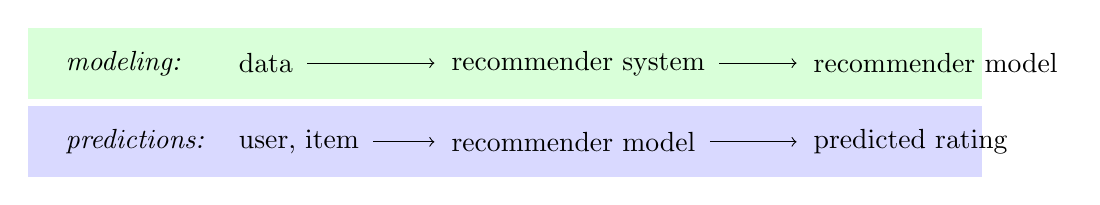
\begin{tikzpicture}[shorten >=1pt,->,draw=black, node distance=\layersep]

    \tikzstyle{every pin edge}=[<-,shorten <=2pt]
    \tikzstyle{rmodel}=[rectangle,fill=green!25,minimum size=20pt,inner sep=5pt]
    \tikzstyle{emodel}=[rectangle,fill=blue!25,minimum size=20pt,inner sep=5pt]
    \tikzstyle{amodel}=[rectangle,fill=red!25,minimum size=20pt,inner sep=5pt]
    \tikzstyle{blank}=[rectangle,right,fill=none,minimum size=20pt,inner sep=5pt]
      
    \fill[green!15] (0,1.1) rectangle (\textwidth,2);
    \fill[blue!15] (0,0.1) rectangle (\textwidth,1);
    
    \node[blank] (I2) at (0.3cm,  0.55) {\emph{predictions:}};
    \node[blank] (I1) at (0.3cm,  1.55)  {\emph{modeling:}};
    
    \node[blank] (I2) at (2.5cm, 0.55) {user, item};
    \node[blank] (I1) at (2.5cm, 1.55) {data};
   
    \node[blank] (P2) at (5.2cm, 0.55) {recommender model};
    \node[blank] (P1) at (5.2cm, 1.55) {recommender system};

    \node[blank] (O2) at (9.8cm, 0.55) {predicted rating};
    \node[blank] (O1) at (9.8cm, 1.55) {recommender model};
    
    \path (I1) edge (P1);
    \path (I2) edge (P2);

    \path (P1) edge (O1);
    \path (P2) edge (O2);
       
  \end{tikzpicture}

  \vspace{1em}
  \caption[Simplified Recommender System]{
    A simplified view of recommender systems:
    Ratings of items by users are used to create a \emph{model}.
    This model is then used to predict unknown ratings between users and items.
    Note that many recommender systems work differently,
    as we shall see later in this thesis.
  }
  \label{fig:simple-rs}
\end{figure}


Consider this: 
when an algorithm is selected for use in a recommender system,
there is a concious decision of which predictive data pattern to use.
Before any user modeling is performed, the researcher or developer selects
one or more methods that is thought to best model every user and item in the system.
While the methods themselves may perform well, their selection
reflects how whoever created the system assumes how each user
can and \emph{should} be modeled. This underlying subjectivity is not desirable.
We call this the \emph{latent subjectivity problem}.

Examples are not hard to come by.
For instance, while one user might appreciate social
influence in their search results, another user might not.
While one user might find frequency of communication maps well to relevance,
another might not. 
One user may think the similarity of movie titles is a good predictor,
while another might be more influenced by their production year.
Some users may favor items rated highly on a global scale,
while others are more interested in what users similar to themselves have to say.

The same problem exists for items. 
For example, while one item might best be judged by its content,
another might be better described by previous ratings from other users.
One item's relevance may be closely tied to when it was created,
while other items may be timeless.
The exact differences are not important, only that they exist.

Another way to put this is that 
\emph{recommender systems methods are dependent on the subjective assumptions of their creators}.
A recommendation method use certain aspects of available data to make predictions,
and these aspects are chosen by whoever creates the system.

Modern aggregation approaches face the same problem. 
Aggregation is done on a generalized, global level,
where each user and item is expected to place the same importance on each modeling method.
While aggregation is selected to minimize some error over a testing set,
the subjective nature remains. The compiled aggregation is a generalization,
treating all users and items the same --- hardly a goal of user modeling.

Should it not be up to the users to implicitly decide which method best describes their preferences?
And, considering the vast scope of items we can come by, will the selected
methods really perform optimally for every item?
We believe the priority of each algorithm should be implicitly and automatically
based on how well they have previously worked for individual users and items.
Without this adaptability, it may be hard for recommender systems
to perform well in scenarios with widely differing users and items.
The scope of users and items is simply too great for any one or generalized combination
of methods to capture the nuanced nature of relevance prediction.

We propose a novel method that we call \emph{adaptive recommenders}, 
where the selection of algorithms is implicitly made by the users and items.
This provides an extra level of abstraction and personalization.
The selection decisions are implicit, and happens in the background, without any extra interaction required.
This leaves the subjective nature of selecting ways to model users and items where it should be.
That is, in the hands of individual users, and dependent on specific items.

This adaptive selection has an important consequence. 
If an algorithm is contextually used based on how well it performs,
any possibly useful recommender algorithm suddenly becomes a worthy addition.
Algorithms are only used in situations they work well.
Those that do not will be used in other situations where they might be better suited.

As far as we know, this kind of adaptive prediction aggregation has not been done before.
The main research question of this thesis is whether or not adaptive recommenders
can outperform traditional approaches.

\hr

\noindent
This thesis is structured as follows.
Chapter \ref{chap:theory} will present background theory and previous work for
the information overload problem, recommender systems, 
prediction aggregation (combining scores) and rank aggregation (combining sorted lists). 
We will also briefly introduce the topics of information
retrieval and personalized search, that will serve
as a case study in later chapters.

Chapter \ref{chap:methods} will further discuss the latent subjectivity problem,
and build the \emph{adaptive recommenders} approach from the ground up.
We will show how this approach can be used for both prediction aggregation
and rank aggregation.

Chapter \ref{chap:results} will test three hypotheses and experiment with our newly built method.
We will experiment with prediction aggregating for singular items, and explore rank aggregation for personalized search.
Finally, Chapter \ref{chap:discussion} will discuss the implications of our results,
important limitations, contributions and suggest future work.

